\documentclass[12pt]{article}

% --- Packages ---
\usepackage[margin=1in]{geometry}
\usepackage[T1]{fontenc}
\usepackage{lmodern}
\usepackage{amsmath, amssymb, amsthm}
\usepackage{graphicx}
\usepackage{booktabs}
\usepackage{hyperref}
\usepackage{float}
\usepackage{natbib}
\usepackage{xcolor}

\hypersetup{
    colorlinks=true,
    linkcolor=blue!60!black,
    citecolor=blue!60!black,
    urlcolor=blue!60!black
}

\title{Bayesian Analysis of Bike Sharing Demand:\\
A Poisson--Gamma Conjugate Framework}
\author{Brian Butler}
\date{February 2026}

\begin{document}
\maketitle

% ==================================================================
\begin{abstract}
This report presents a Bayesian analysis of hourly bike rental demand
using the UCI Bike Sharing Dataset \citep{fanaee2013}.  We begin with
a homogeneous Poisson likelihood and derive the maximum likelihood
estimator in closed form.  A conjugate Gamma prior yields a tractable
posterior whose predictive distribution is Negative Binomial.  We
define an ``overload'' event, compute posterior predictive overload
probabilities, and apply calibration techniques (Platt scaling,
isotonic regression) to improve probabilistic accuracy.  Cost-based
and constraint-based threshold policies are derived and evaluated.
The homogeneous model is shown to be fundamentally inadequate---its
predictive probabilities are constant across hours, producing
degenerate alert policies.  A stratified model that conditions on
hour-of-day and workday status demonstrates substantial improvement,
and we discuss further extensions via Poisson regression with
covariates.
\end{abstract}

% ==================================================================
\section{Introduction and Data Acquisition}
\label{sec:intro}

The Capital Bikeshare system in Washington, D.C.\ records the number
of bicycles rented each hour.  Understanding and predicting demand is
operationally important: if the system can anticipate high-demand
hours, it can pre-position bicycles, schedule maintenance during
lulls, and issue overload alerts to managers.

We use the hourly subset of the UCI Bike Sharing Dataset
\citep{fanaee2013}, which contains $T = 17{,}379$ records spanning
January 1, 2011 through December 31, 2012.  Each record includes the
hourly rental count $Y_t$ along with calendar features
(hour, day-of-week, month, holiday, working day) and weather
covariates (temperature, humidity, wind speed, weather situation).

Our analysis proceeds as follows.  Section~\ref{sec:eda} conducts
exploratory analysis.  Section~\ref{sec:poisson} derives the Poisson
MLE.  Section~\ref{sec:posterior} introduces the conjugate
Gamma--Poisson posterior.  Section~\ref{sec:ci} reports credible
intervals.  Section~\ref{sec:predictive} defines the overload event
and computes posterior predictive probabilities.
Section~\ref{sec:calibration} applies calibration techniques.
Section~\ref{sec:threshold} performs threshold selection.
Section~\ref{sec:stratified} introduces a stratified model, and
Section~\ref{sec:discussion} discusses limitations and improvements.

% ==================================================================
\section{Exploratory Data Analysis}
\label{sec:eda}

Table~\ref{tab:summary} presents the basic descriptive statistics of
the hourly counts.

\begin{table}[H]
\centering
\caption{Summary statistics of hourly rental counts $Y_t$.}
\label{tab:summary}
\begin{tabular}{lr}
\toprule
\textbf{Statistic} & \textbf{Value} \\
\midrule
Number of records $T$ & 17,379 \\
Time span & 2011-01-01 to 2012-12-31 \\
Sample mean $\bar{Y}$ & 189.46 \\
Sample variance $s^2$ & 32,899.57 \\
Variance / Mean ratio & 173.65 \\
\bottomrule
\end{tabular}
\end{table}

The variance-to-mean ratio of approximately 174 provides the first
clear signal that a simple Poisson model---which requires
$\text{Var}(Y) = E[Y]$---is wholly inadequate.  This massive
\emph{overdispersion} arises from the heterogeneous nature of demand:
hourly counts range from near zero (late-night hours) to over 900
(peak commuting hours).

Figure~\ref{fig:timeseries} displays the first four weeks of data,
revealing pronounced daily periodicity.  Workdays exhibit sharp
bimodal peaks during commute hours (approximately 8\,AM and 5--6\,PM),
while weekends show a single broad midday plateau.  Night-time counts
fall to near zero regardless of day type.

\begin{figure}[H]
\centering
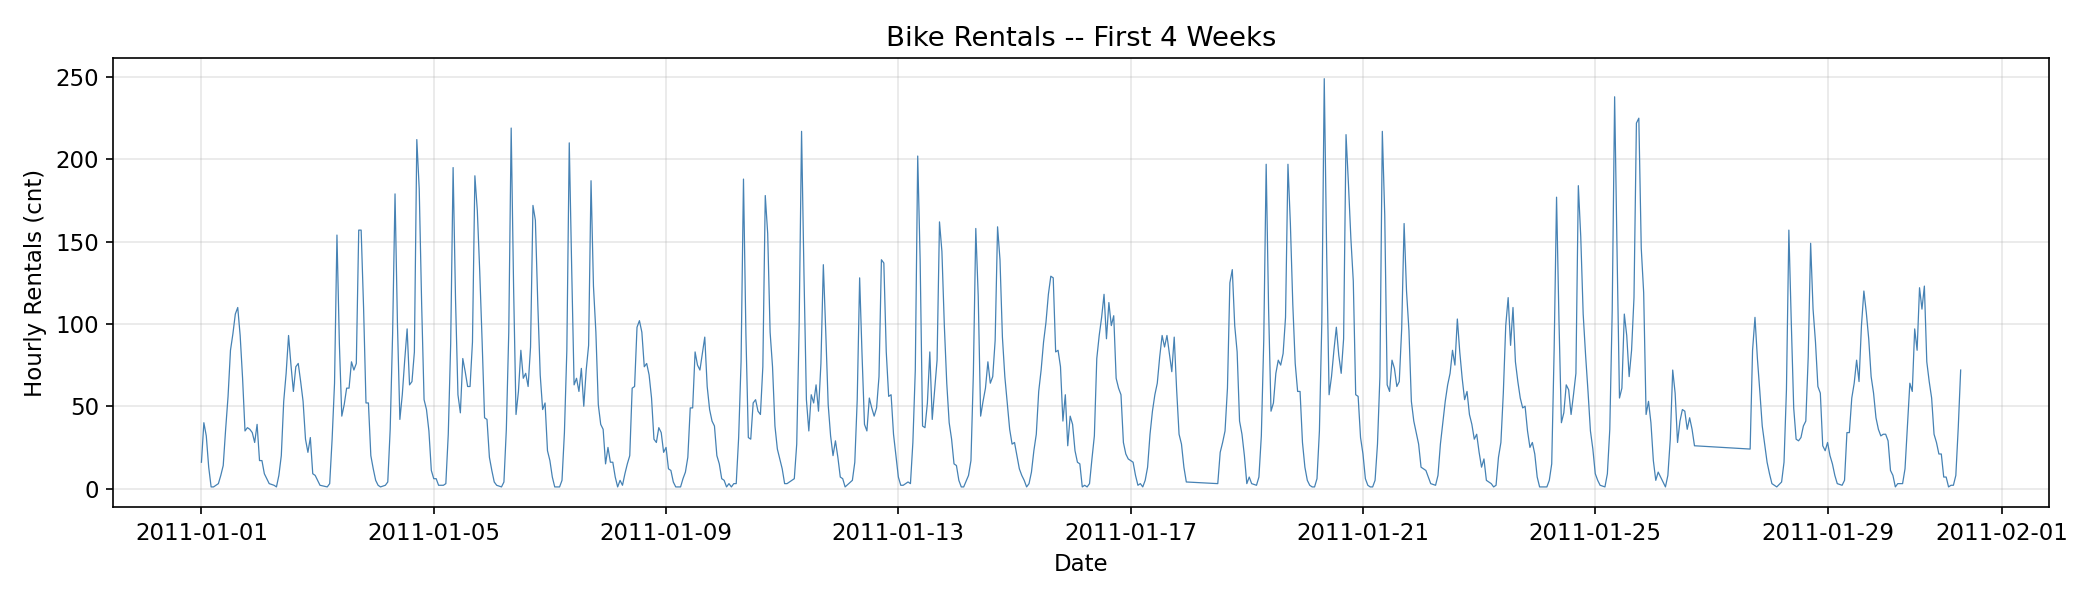
\includegraphics[width=\textwidth]{fig1_timeseries.png}
\caption{Hourly bike rentals for the first four weeks of the dataset.
  The strong daily periodicity and workday commute peaks are clearly
  visible.}
\label{fig:timeseries}
\end{figure}

Figure~\ref{fig:histogram} shows the marginal distribution of hourly
counts.  The histogram is heavily right-skewed with a mode near zero
and a long right tail extending past 900 rentals---far from the
near-symmetric bell shape that a Poisson distribution with
$\lambda \approx 189$ would produce.

\begin{figure}[H]
\centering
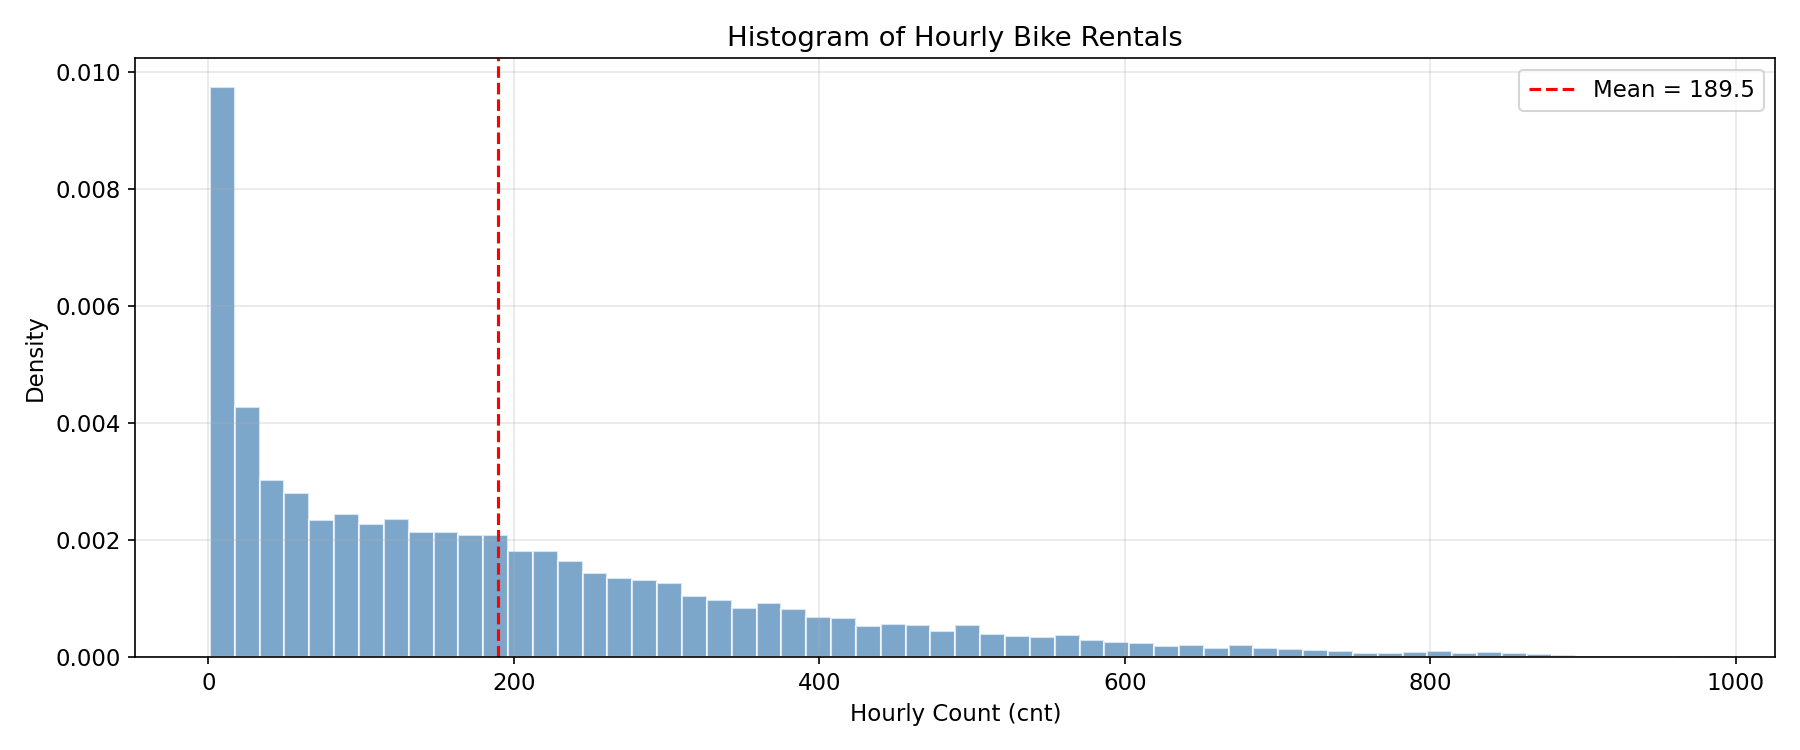
\includegraphics[width=0.8\textwidth]{fig2_histogram.png}
\caption{Histogram of hourly rental counts.  The red dashed line marks
  the sample mean $\bar{Y} = 189.5$.  The heavy right skew and the
  concentration of mass near zero are inconsistent with a homogeneous
  Poisson model.}
\label{fig:histogram}
\end{figure}

% ==================================================================
\section{Poisson Likelihood and Maximum Likelihood Estimation}
\label{sec:poisson}

We begin by treating the counts $Y_1, \dots, Y_T$ as i.i.d.\
draws from a Poisson distribution with unknown rate $\lambda > 0$:
\begin{equation}
Y_t \mid \lambda \;\stackrel{\text{iid}}{\sim}\; \text{Poisson}(\lambda),
\qquad t = 1, \dots, T.
\end{equation}

The likelihood function is
\begin{equation}
L(\lambda \mid \mathbf{y}) = \prod_{t=1}^{T}
  \frac{\lambda^{y_t} e^{-\lambda}}{y_t!}
= \frac{\lambda^{\,\sum_t y_t}\, e^{-T\lambda}}{\prod_t y_t!}\,.
\end{equation}

The log-likelihood (dropping the constant $\sum_t \ln(y_t!)$) is
\begin{equation}
\ell(\lambda) = \Bigl(\sum_{t=1}^{T} y_t\Bigr) \ln \lambda - T\lambda.
\end{equation}

Setting $d\ell/d\lambda = 0$:
\begin{equation}
\frac{\sum_t y_t}{\lambda} - T = 0
\quad\Longrightarrow\quad
\hat{\lambda}_{\mathrm{mle}} = \frac{1}{T}\sum_{t=1}^{T} y_t = \bar{Y}.
\end{equation}

Numerically, $\sum y_t = 3{,}292{,}679$ and $T = 17{,}379$, giving
\begin{equation}
\hat{\lambda}_{\mathrm{mle}} = 189.4631.
\end{equation}

This estimate captures the overall average demand but treats every
hour identically---it cannot distinguish a 3\,AM lull from a 5\,PM
rush.

% ==================================================================
\section{Gamma Prior and Conjugate Posterior}
\label{sec:posterior}

The Gamma distribution is conjugate to the Poisson likelihood.  We
place a weakly informative prior on $\lambda$:
\begin{equation}
\lambda \sim \text{Gamma}(\alpha_0, \beta_0),
\quad \alpha_0 = 2,\;\; \beta_0 = 0.01,
\end{equation}
using the shape/rate parameterisation so that the prior mean is
$\alpha_0/\beta_0 = 200$ and the prior variance is
$\alpha_0/\beta_0^2 = 20{,}000$.  This prior is deliberately
diffuse, expressing only a vague belief that demand is on the order
of hundreds per hour.

The conjugate posterior is
\begin{equation}
\lambda \mid \mathbf{y} \;\sim\;
\text{Gamma}\!\bigl(\alpha_0 + \textstyle\sum y_t,\;\;
\beta_0 + T\bigr).
\label{eq:posterior}
\end{equation}

Substituting the data:
\begin{align}
\alpha_{\text{post}} &= 2 + 3{,}292{,}679 = 3{,}292{,}681, \\
\beta_{\text{post}} &= 0.01 + 17{,}379 = 17{,}379.01.
\end{align}

The posterior mean is
\begin{equation}
E[\lambda \mid \mathbf{y}]
= \frac{\alpha_{\text{post}}}{\beta_{\text{post}}}
= 189.4631,
\end{equation}
which differs from the MLE by only $6 \times 10^{-6}$---confirming
that the prior is overwhelmed by the data.

\paragraph{Shrinkage interpretation.}
The posterior mean can be decomposed as a weighted average of the
prior mean and the MLE:
\begin{equation}
E[\lambda \mid \mathbf{y}]
= \underbrace{\frac{\beta_0}{\beta_0 + T}}_{\approx\, 10^{-6}}
  \cdot \frac{\alpha_0}{\beta_0}
\;+\; \underbrace{\frac{T}{\beta_0 + T}}_{\approx\, 1}
  \cdot \bar{Y}.
\end{equation}
The weight on the prior mean is negligible (${\sim}10^{-6}$).
Intuitively, $\alpha_0 = 2$ pseudo-counts from $\beta_0 = 0.01$
pseudo-hours of imaginary data are overwhelmed by $T = 17{,}379$ real
hours.

% ==================================================================
\section{95\% Credible Interval}
\label{sec:ci}

The 95\% equal-tailed credible interval is obtained from the quantile
function of the Gamma$(\alpha_{\text{post}},\, \beta_{\text{post}})$
posterior:
\begin{equation}
\Pr\!\bigl[\,189.2585 \;\le\; \lambda \;\le\; 189.6678 \;\bigm|\;
\mathbf{y}\,\bigr] = 0.95.
\end{equation}

The interval width is approximately 0.41 rentals per hour---extremely
narrow because $T = 17{,}379$ observations concentrate the posterior
tightly around $\bar{Y}$.

\begin{figure}[H]
\centering
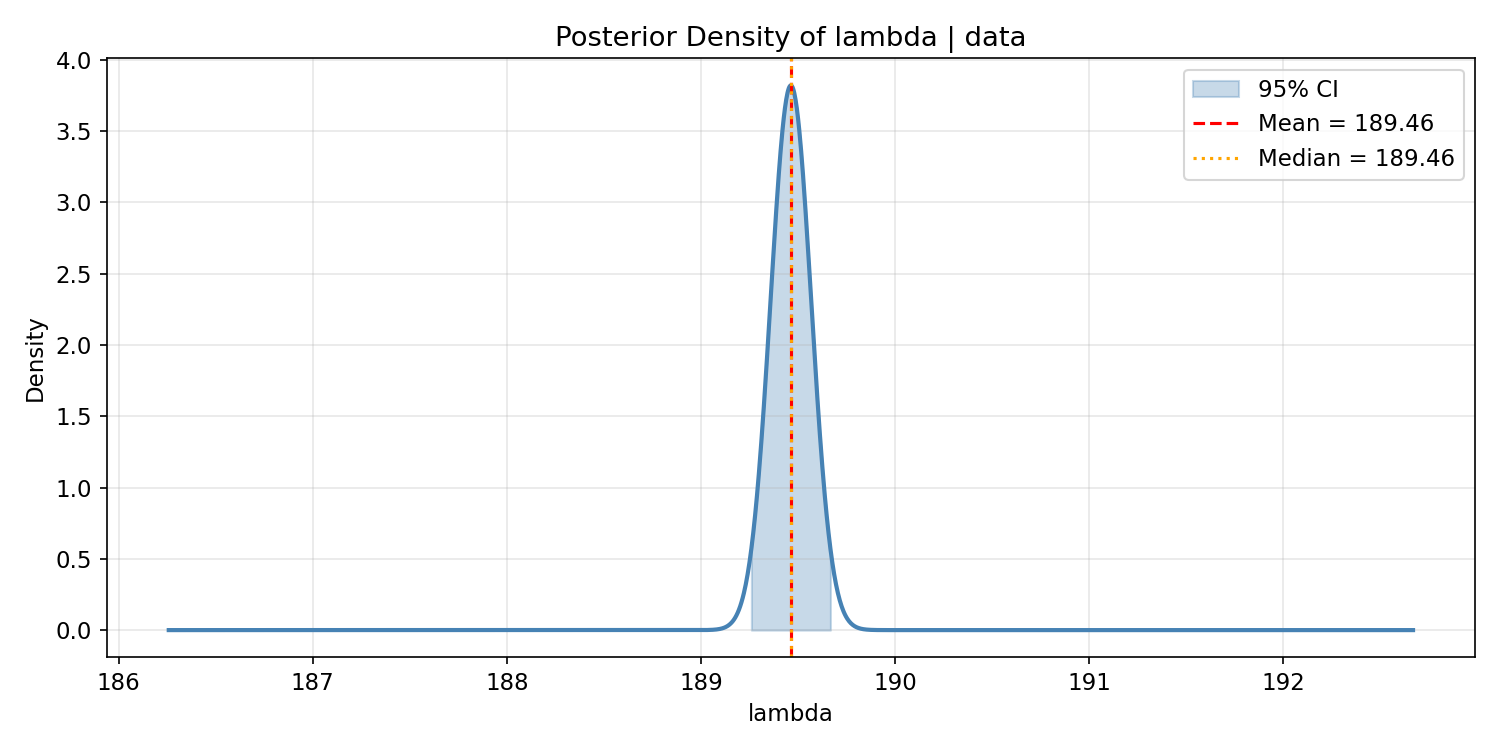
\includegraphics[width=0.85\textwidth]{fig4_posterior.png}
\caption{Posterior density $p(\lambda \mid \mathbf{y})$ with the 95\%
  credible interval (shaded region), posterior mean (red dashed), and
  median (orange dotted).  The density is extremely concentrated due
  to the large sample size.}
\label{fig:posterior}
\end{figure}

% ==================================================================
\section{Posterior Predictive Distribution and Overload Alert}
\label{sec:predictive}

\subsection{Data Splitting}

We partition the data chronologically into training (70\%, $n_{\text{train}} = 12{,}165$),
validation (15\%, $n_{\text{val}} = 2{,}606$), and test (15\%,
$n_{\text{test}} = 2{,}608$) sets.  The training set fits the model,
the validation set tunes calibration and thresholds, and the test set
provides final, unbiased evaluation.

\subsection{Overload Event}

We define an \emph{overload} event as any hour $t$ where the rental
count exceeds the 90th percentile of training counts:
\begin{equation}
A_t = \mathbf{1}(Y_t > L),
\qquad L = 380.
\end{equation}

The overload base rate is 29.2\% on the validation set and 21.8\% on
the test set.

\subsection{Posterior Predictive Probability}

Given the conjugate posterior~\eqref{eq:posterior}, the one-step-ahead
predictive distribution is Negative Binomial:
\begin{equation}
Y_{t+1} \mid \mathbf{y}_{1:t}
\;\sim\;
\text{NegBin}\!\Bigl(n = \alpha_{\text{post}},\;\;
p = \frac{\beta_{\text{post}}}{\beta_{\text{post}} + 1}\Bigr).
\end{equation}

The overload probability for each hour is therefore
\begin{equation}
p_t = \Pr(Y_t > L \mid \mathbf{y}_{1:t-1})
= 1 - F_{\text{NB}}(L;\, \alpha_{\text{post}},\, p),
\end{equation}
where $F_{\text{NB}}$ is the Negative Binomial CDF and the posterior
parameters are updated sequentially as each new observation arrives.

\begin{figure}[H]
\centering
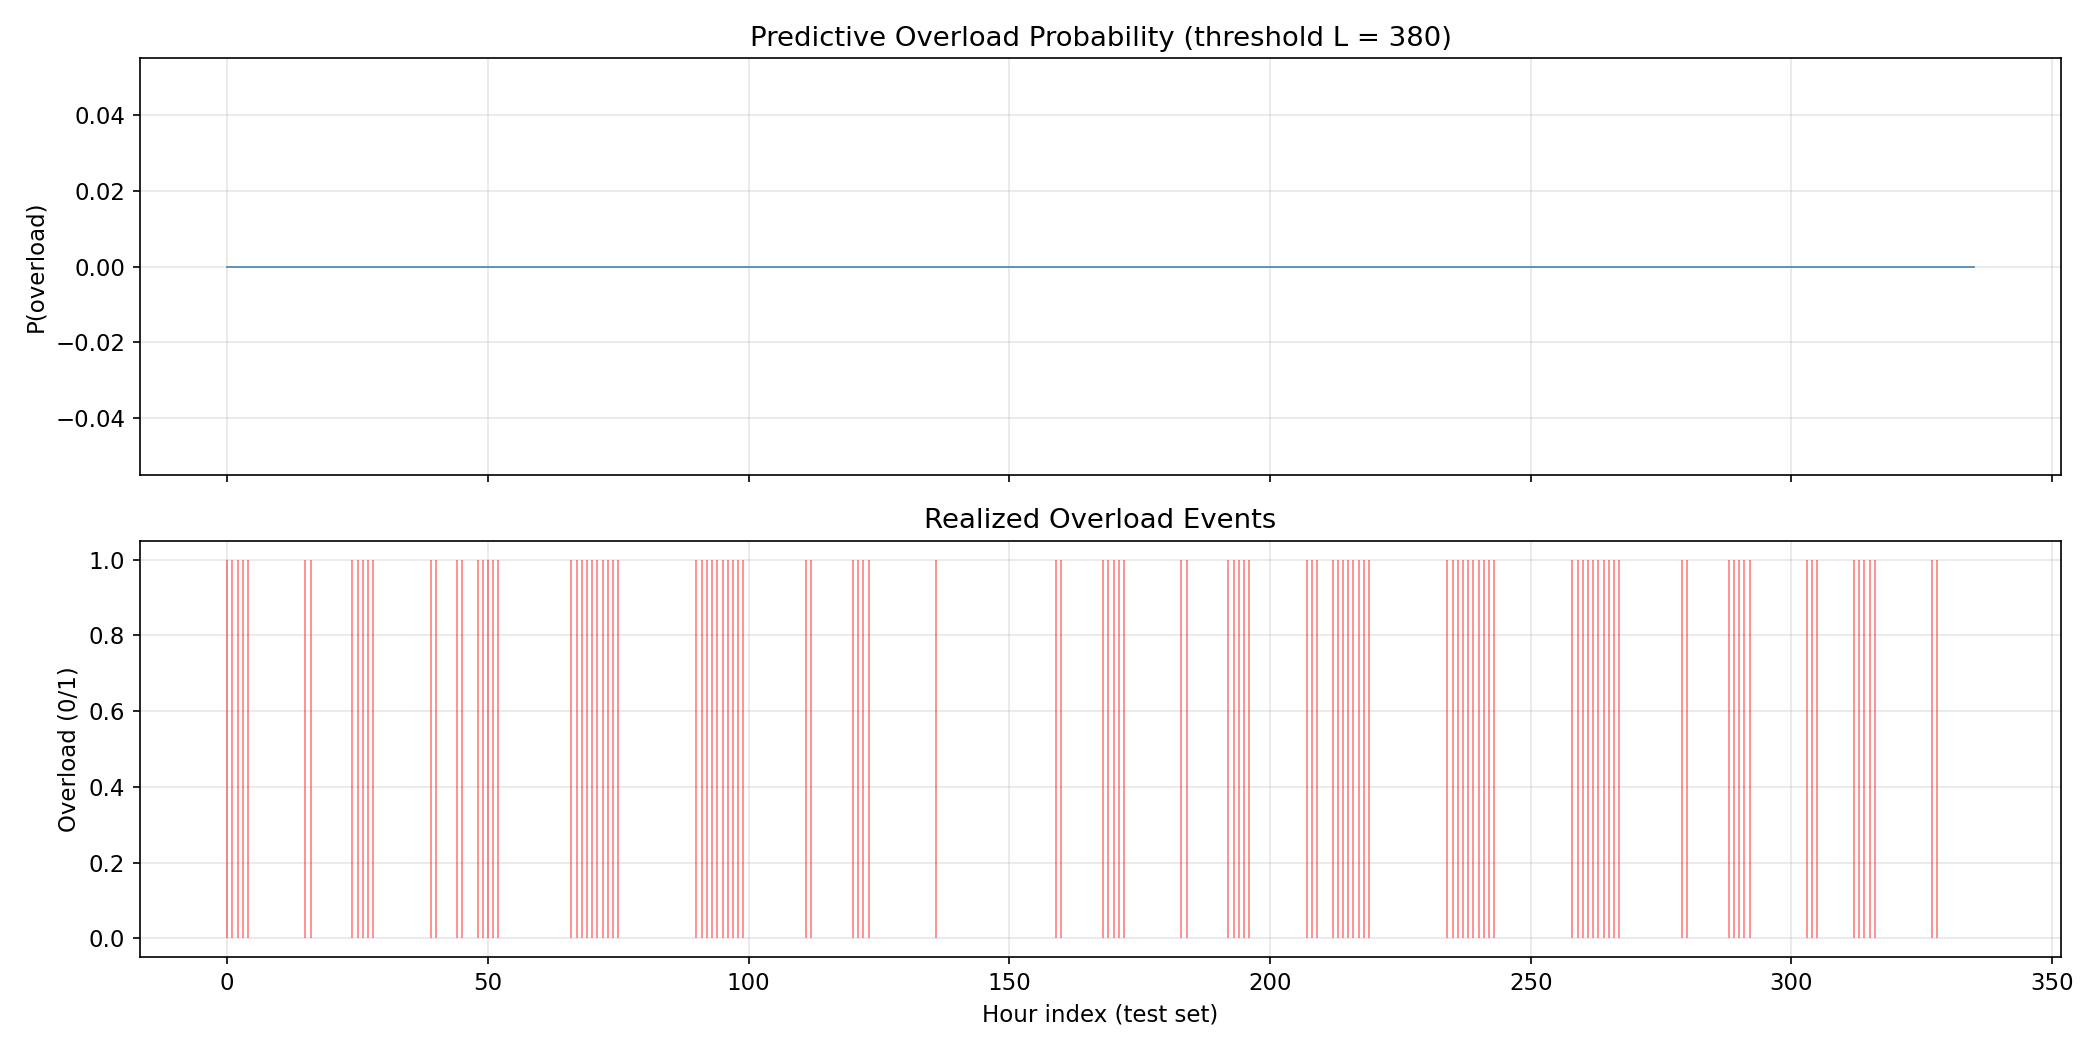
\includegraphics[width=\textwidth]{fig5_predictive.png}
\caption{Top: posterior predictive overload probability $p_t$ for the
  first two weeks of the test set.  Bottom: realized overload events
  (red vertical lines where $Y_t > 380$).  Under the homogeneous
  model, all hours receive essentially the same predicted probability,
  providing no ability to discriminate high-demand from low-demand
  periods.}
\label{fig:predictive}
\end{figure}

The constant-$\lambda$ model assigns nearly identical overload
probabilities to every hour---whether it is 3\,AM or 5\,PM---because
the posterior is concentrated around a single $\lambda \approx 189$,
and $\Pr(Y > 380 \mid \lambda = 189)$ is the same for all hours.

% ==================================================================
\section{Calibration}
\label{sec:calibration}

Although the homogeneous model lacks discrimination (it cannot rank
hours by overload risk), we still assess its \emph{calibration}:
whether predicted probabilities match observed frequencies.  A model
can be well-calibrated without discriminating (e.g., always predicting
the base rate), and it can discriminate well without being calibrated
(e.g., correct rankings but wrong probability magnitudes).

We apply two standard post-hoc calibration techniques, both fit on the
validation set:

\begin{itemize}
\item \textbf{Platt scaling:} a logistic regression of the binary
  outcome $A_t$ on the raw score $p_t$, which learns a sigmoid
  remapping.
\item \textbf{Isotonic regression:} a non-parametric, monotone
  step-function fit of $A_t$ on $p_t$.
\end{itemize}

\begin{table}[H]
\centering
\caption{Brier scores on the test set (lower is better).}
\label{tab:brier}
\begin{tabular}{lc}
\toprule
\textbf{Method} & \textbf{Brier Score} \\
\midrule
Raw (posterior predictive) & 0.2182 \\
Platt scaling              & 0.1761 \\
Isotonic regression        & 0.1761 \\
\bottomrule
\end{tabular}
\end{table}

The raw Brier score (0.2182) is essentially equal to the overload
base rate, confirming that the model provides \emph{no useful
probabilistic information} beyond predicting the marginal frequency
for every hour.  Platt scaling and isotonic regression reduce the
score modestly by correcting the probability mapping, but they cannot
create discrimination where none exists.

\begin{figure}[H]
\centering
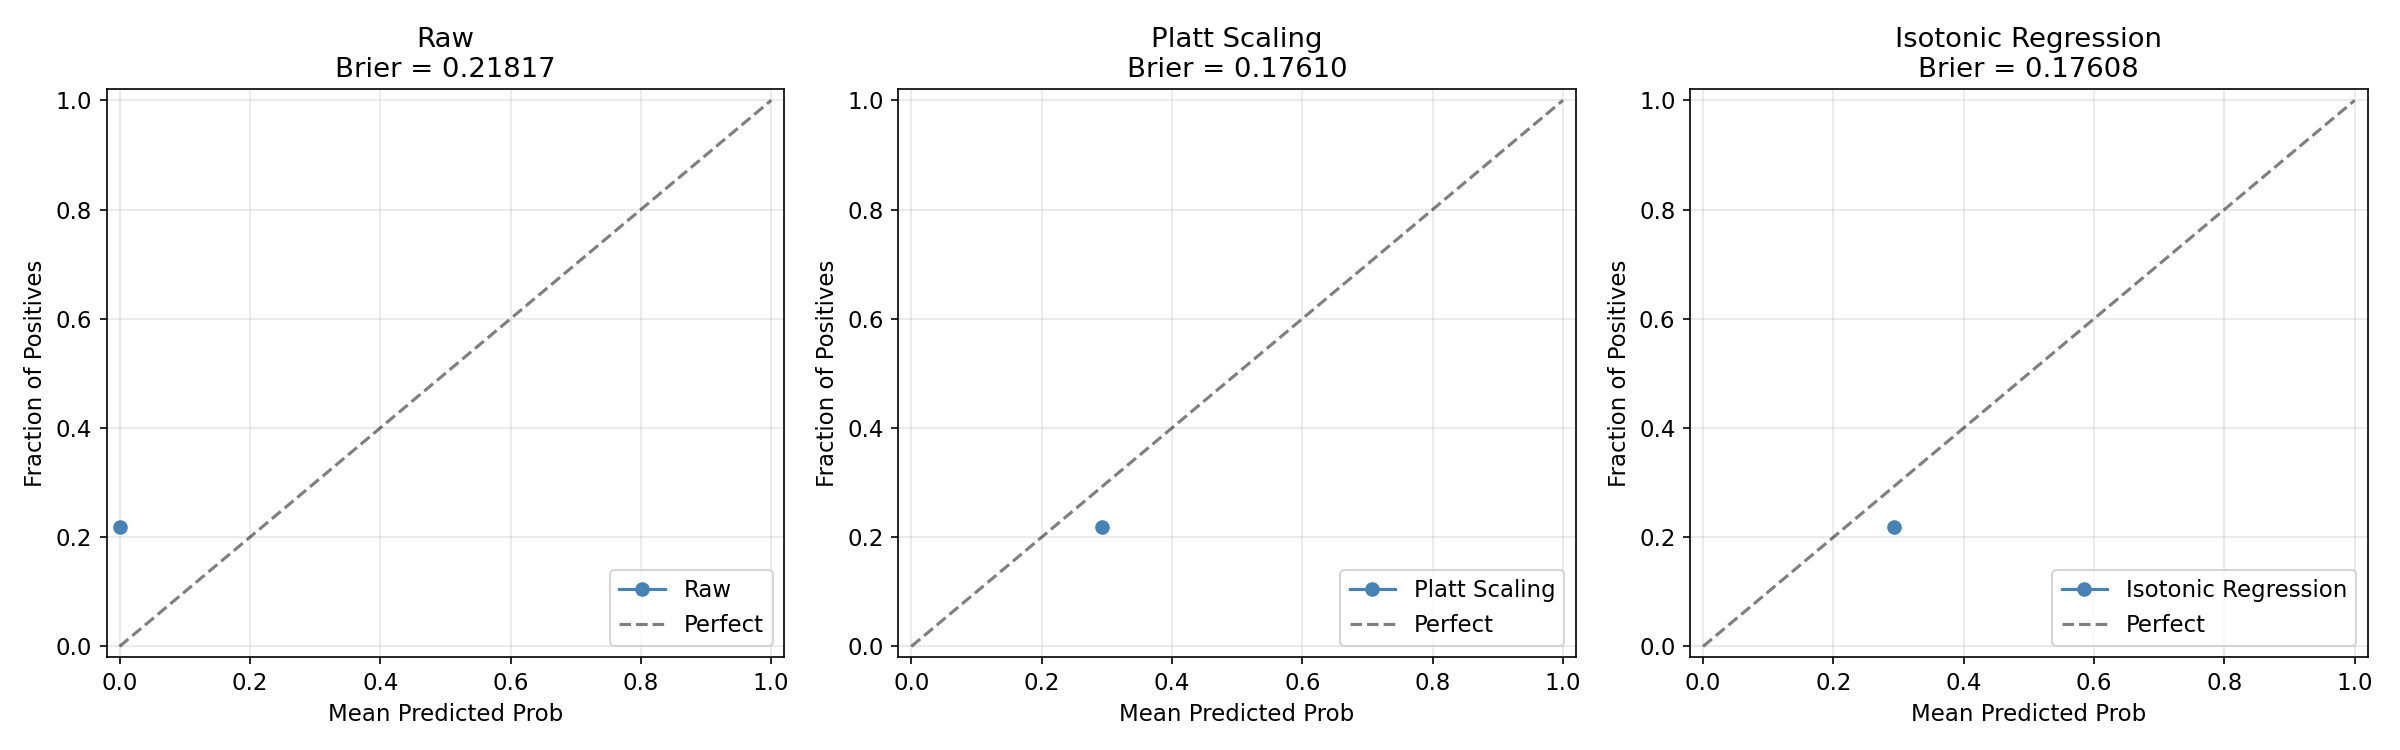
\includegraphics[width=\textwidth]{fig6_calibration.png}
\caption{Reliability diagrams (calibration curves) for the raw,
  Platt-scaled, and isotonic-calibrated overload probabilities.  A
  perfectly calibrated model follows the diagonal.  The Brier score
  for each method is indicated in the subplot title.}
\label{fig:calibration}
\end{figure}

% ==================================================================
\section{Threshold Selection}
\label{sec:threshold}

To operationalise the overload alert, we convert the continuous
probability $p_t$ into a binary decision: fire an alert when
$p_t \ge \tau$.  We consider two approaches to choosing $\tau$.

\subsection{Cost-Based Threshold}

We assign asymmetric misclassification costs---missing a genuine
overload ($C_{\mathrm{fn}} = 10$) is ten times worse than a false
alarm ($C_{\mathrm{fp}} = 1$):
\begin{equation}
\text{Expected Cost}
= \frac{1}{n}\bigl[C_{\mathrm{fp}} \cdot \text{FP}
  + C_{\mathrm{fn}} \cdot \text{FN}\bigr].
\end{equation}

The optimal $\tau$ is selected on the validation set by minimising this
cost over a fine grid.

\subsection{Constraint-Based Threshold}

Alternatively, we require that the false-alert rate not exceed 5\%:
\begin{equation}
\text{FAR} = \frac{\text{FP}}{\text{FP} + \text{TN}} \le 0.05,
\end{equation}
and subject to this constraint, we choose the lowest $\tau$ (i.e.,
maximise recall).

\subsection{Homogeneous Model Results}

\begin{table}[H]
\centering
\caption{Threshold selection results on the test set
  (homogeneous model with isotonic calibration).}
\label{tab:threshold_homo}
\begin{tabular}{lcc}
\toprule
& \textbf{Cost-Based} & \textbf{Constraint-Based} \\
\midrule
Threshold $\tau$ & 0.001 & 0.999 \\
TP / FP / FN / TN & 569 / 2039 / 0 / 0 & 0 / 0 / 569 / 2039 \\
Precision & 0.218 & --- \\
Recall & 1.000 & 0.000 \\
False-alert rate & 1.000 & 0.000 \\
Expected cost/hour & 0.782 & --- \\
\bottomrule
\end{tabular}
\end{table}

\begin{figure}[H]
\centering
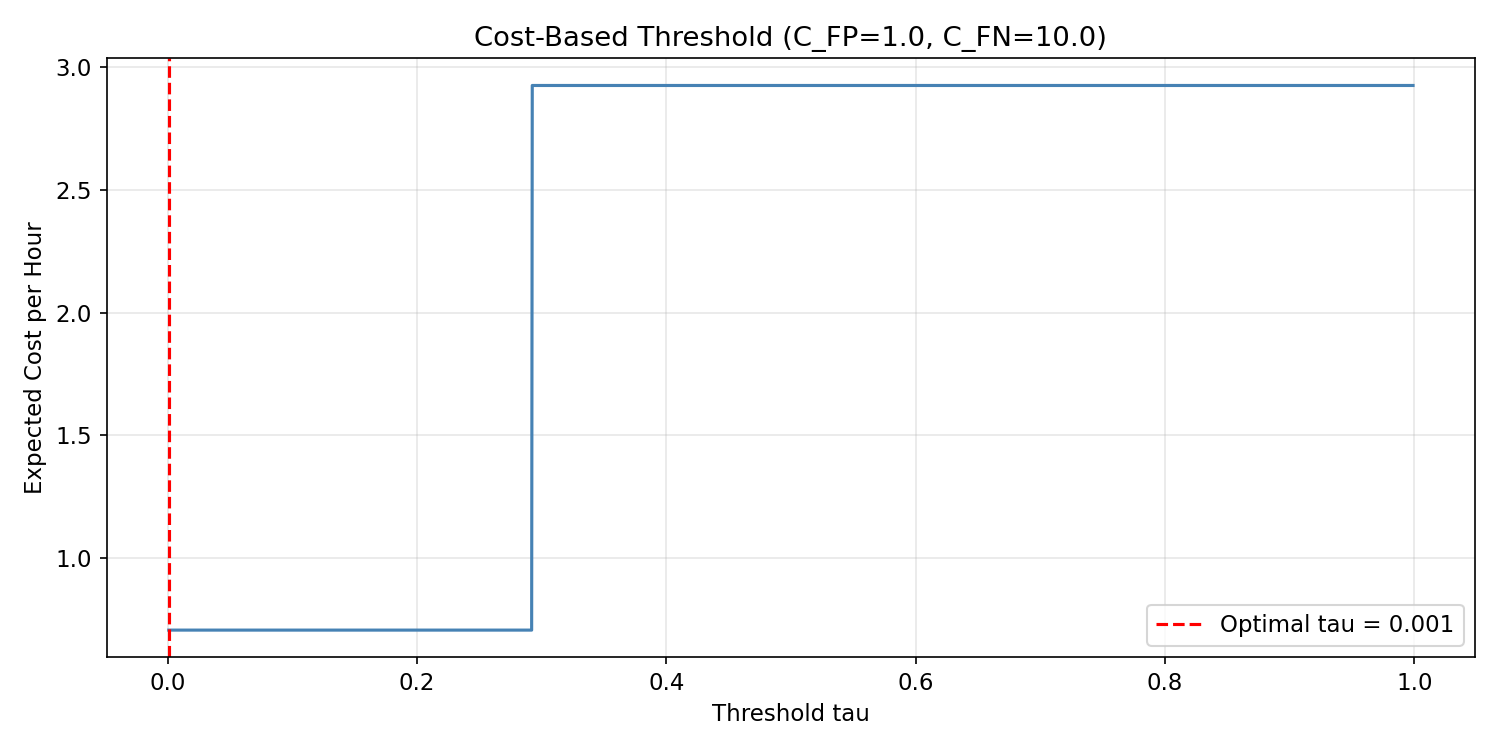
\includegraphics[width=0.85\textwidth]{fig7a_cost_curve.png}
\caption{Expected cost per hour as a function of the decision
  threshold~$\tau$ (homogeneous model).  Because the predicted
  probabilities are nearly identical for all hours, the cost curve is
  essentially a step function with no informative interior minimum.}
\label{fig:cost_homo}
\end{figure}

The results are \emph{degenerate}.  The cost-based approach sets
$\tau \approx 0$, alerting on every single hour (precision = 0.22,
recall = 1.0).  The constraint-based approach sets $\tau \approx 1$,
issuing no alerts whatsoever (recall = 0).  There is no useful
threshold between these extremes because the homogeneous model assigns
essentially the same overload probability to every hour.

% ==================================================================
\section{Stratified Model: Hour $\times$ Workday}
\label{sec:stratified}

\subsection{Approach}

The failure of the homogeneous model motivates conditioning on the two
most important demand drivers: \textbf{hour of day} (0--23) and
\textbf{workday status} (binary).  This yields $24 \times 2 = 48$
strata, each receiving its own independent conjugate Gamma--Poisson
posterior:
\begin{equation}
\lambda_s \mid \mathbf{y}_s
\;\sim\;
\text{Gamma}\!\bigl(\alpha_0 + \textstyle\sum_{t \in s} y_t,\;\;
\beta_0 + n_s\bigr),
\qquad s = 1, \dots, 48,
\end{equation}
where $n_s$ is the number of training hours in stratum $s$.  Each
stratum's predictive distribution is then a stratum-specific Negative
Binomial:
\begin{equation}
p_t^{(s)} = 1 - F_{\text{NB}}\!\bigl(L;\; \alpha_s,\;
\beta_s / (\beta_s + 1)\bigr).
\end{equation}

Peak-demand strata (e.g., workday 5--6\,PM) produce high predicted
overload probabilities, while off-peak strata (e.g., 3\,AM) produce
values near zero---giving the model genuine discrimination.

\subsection{Results}

\begin{table}[H]
\centering
\caption{Brier score comparison: homogeneous vs.\ stratified model.}
\label{tab:brier_compare}
\begin{tabular}{lcc}
\toprule
\textbf{Method} & \textbf{Homogeneous} & \textbf{Stratified} \\
\midrule
Raw & 0.2182 & 0.1554 \\
Platt scaling & 0.1761 & 0.1372 \\
Isotonic regression & 0.1761 & 0.1110 \\
\bottomrule
\end{tabular}
\end{table}

The stratified model reduces the Brier score by 29\% (raw) and 37\%
(after isotonic calibration), confirming substantially improved
probabilistic accuracy.

\begin{figure}[H]
\centering
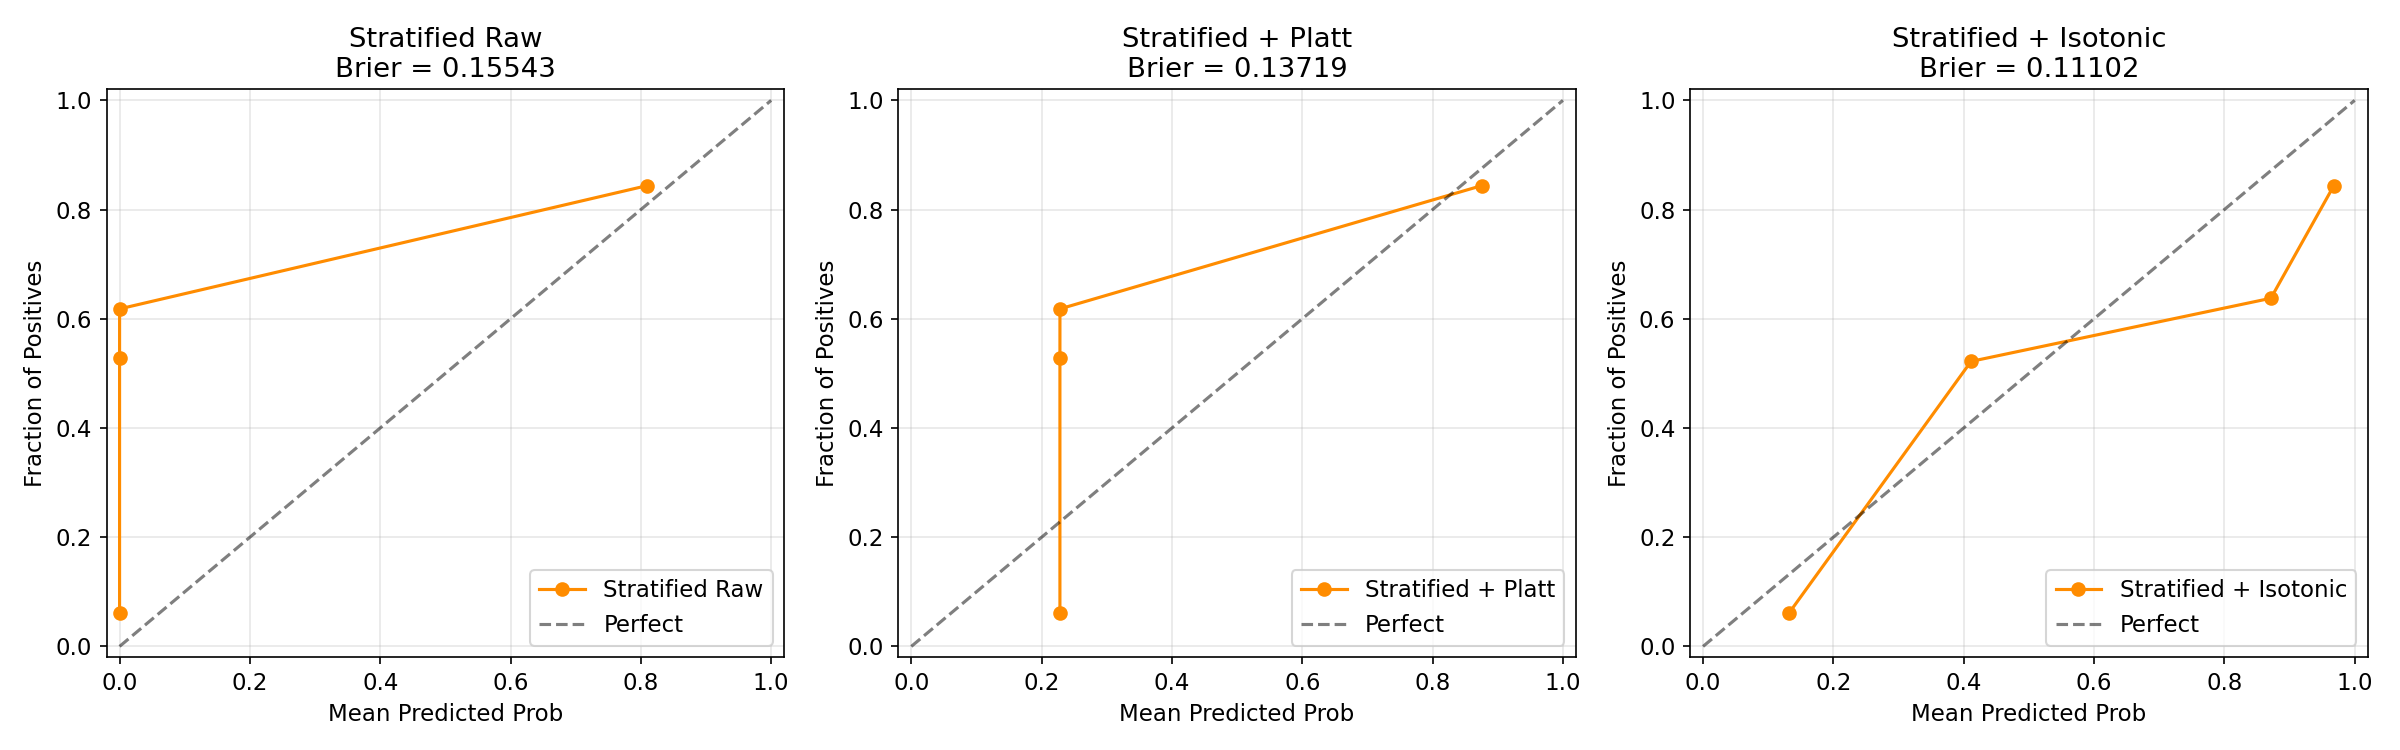
\includegraphics[width=\textwidth]{fig8a_calibration_stratified.png}
\caption{Reliability diagrams for the stratified model (raw,
  Platt-scaled, and isotonic-calibrated probabilities).  Compared to
  Figure~\ref{fig:calibration}, the curve tracks the diagonal far
  more closely, indicating both improved discrimination and
  calibration.}
\label{fig:cal_strat}
\end{figure}

\subsection{Threshold Selection---Stratified Model}

\begin{table}[H]
\centering
\caption{Full comparison of threshold selection results
  on the test set.}
\label{tab:compare_full}
\begin{tabular}{lcc}
\toprule
\textbf{Metric} & \textbf{Homogeneous} & \textbf{Stratified} \\
\midrule
Brier score (raw) & 0.2182 & \textbf{0.1554} \\
Brier score (calibrated) & 0.1761 & \textbf{0.1110} \\
Cost-based $\tau$ & 0.001 & 0.001 \\
Cost-based precision & 0.218 & \textbf{0.868} \\
Cost-based recall & 1.000 & 0.336 \\
Cost-based exp.\ cost/hour & \textbf{0.782} & 1.461 \\
Constraint $\tau$ (FAR $\le$ 5\%) & 0.999 & 0.999 \\
Constraint recall & 0.000 & 0.000 \\
\bottomrule
\end{tabular}
\end{table}

\begin{figure}[H]
\centering
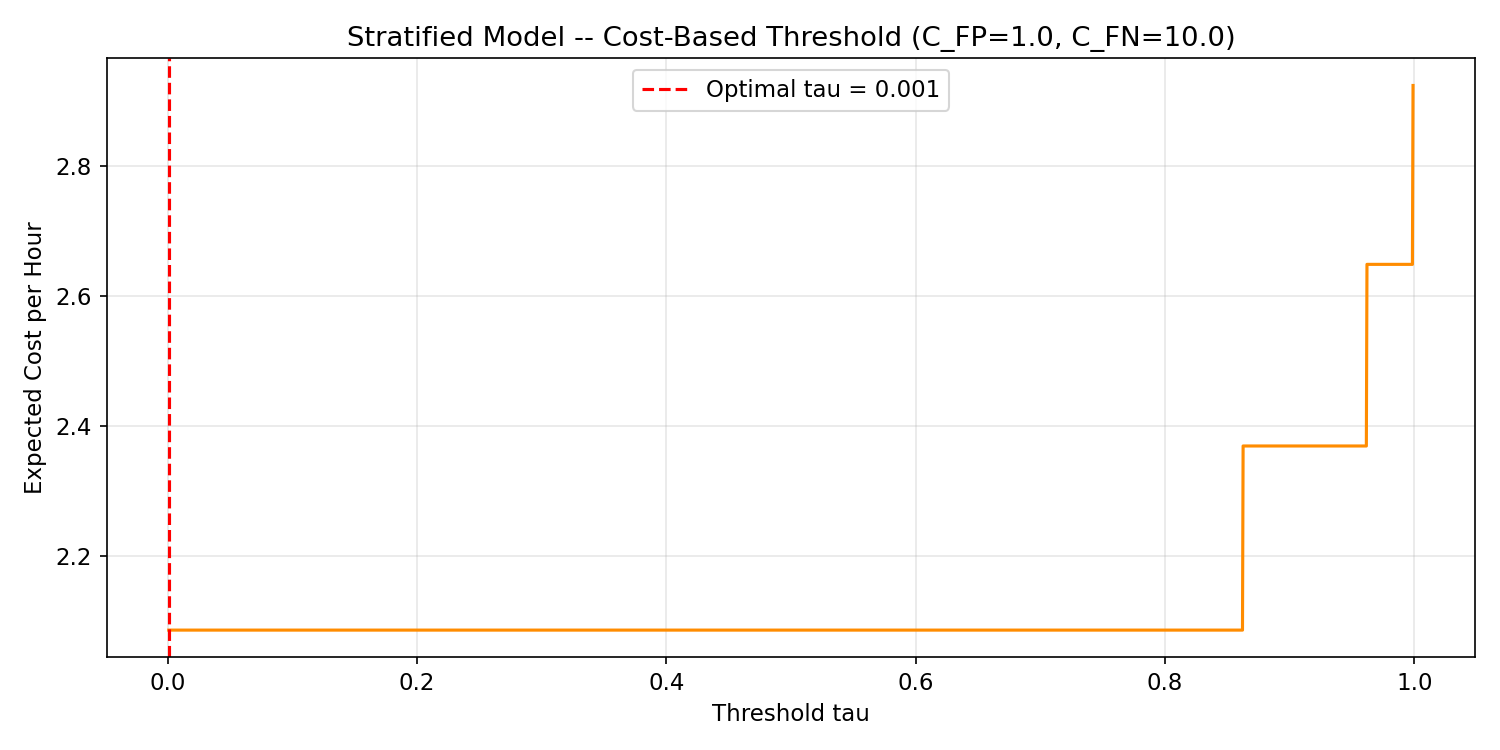
\includegraphics[width=0.85\textwidth]{fig8b_cost_curve_stratified.png}
\caption{Cost curve for the stratified model.  Unlike
  Figure~\ref{fig:cost_homo}, the curve now exhibits a genuine
  trade-off region.}
\label{fig:cost_strat}
\end{figure}

Under the cost-based policy, the stratified model achieves
\textbf{precision = 0.87}: when it fires an alert, it is correct 87\%
of the time.  This is a genuine precision--recall trade-off---far from
the homogeneous model's degenerate ``alert everything'' result.  The
constraint-based threshold remains at $\tau = 0.999$ (zero recall)
because the 48 strata produce only a handful of discrete probability
levels with a large gap between off-peak (${\approx}0$) and peak-hour
(${\approx}0.86$--$0.999$) groups; any threshold below ${\sim}0.86$
triggers false alerts from the high-probability strata.  A
finer-grained model would smooth this probability surface.

% ==================================================================
\section{Discussion}
\label{sec:discussion}

\subsection{Why the Constant-$\lambda$ Model Is Unsatisfactory}

The homogeneous Poisson model suffers from three fundamental problems:

\begin{enumerate}
\item \textbf{Massive overdispersion.}  The Poisson distribution
  requires $\text{Var}(Y) = E[Y]$, yet the observed
  variance-to-mean ratio is 174.  This makes pointwise prediction
  intervals far too narrow and invalidates standard Poisson-based
  inference.

\item \textbf{Ignored heterogeneity.}  Bike demand is driven by
  strong hour-of-day, day-of-week, seasonal, and weather effects.
  Collapsing all 17,379 hours into a single rate $\lambda = 189$
  treats a 3\,AM observation and a 5\,PM observation as
  exchangeable---they are not.

\item \textbf{Zero discrimination.}  Because every hour receives
  the same predicted rate, the posterior predictive overload
  probability $p_t$ is effectively constant.  No threshold on a
  constant score can distinguish overload from non-overload hours,
  producing the degenerate alert policies seen in
  Table~\ref{tab:threshold_homo}.
\end{enumerate}

The stratified model (Section~\ref{sec:stratified}) partially
addresses problems 2 and 3 by conditioning on hour-of-day and workday
status, reducing the Brier score by 37\% and achieving 87\% precision
at the cost-based operating point.  However, it does not model
overdispersion \emph{within} strata, and its coarse (48-level)
probability surface limits fine-grained threshold selection.

\subsection{Improvement Directions}

Several concrete extensions would improve this analysis:

\begin{enumerate}
\item \textbf{Poisson regression with covariates.}  A log-linear
  model of the form
  \begin{equation}
  \ln E[Y_t \mid \mathbf{x}_t] = \mathbf{x}_t^\top \boldsymbol{\beta},
  \end{equation}
  where $\mathbf{x}_t$ includes hour-of-day dummies, day-of-week
  effects, temperature, humidity, and calendar indicators, would
  produce a continuous probability surface rather than the discrete
  48-level structure of the stratified model.

\item \textbf{Negative Binomial regression.}  Replacing the Poisson
  with a Negative Binomial response directly models overdispersion
  via
  \begin{equation}
  Y_t \mid \mu_t, r \;\sim\; \text{NegBin}(\mu_t, r),
  \qquad \text{Var}(Y_t) = \mu_t + \mu_t^2/r,
  \end{equation}
  where $r$ is a dispersion parameter estimated from data.

\item \textbf{Hierarchical Bayesian model.}  Rather than fitting 48
  independent strata, a hierarchical model would share information
  across similar strata (e.g., adjacent hours) via a common
  hyper-prior, improving estimates for strata with fewer observations.

\item \textbf{Temporal dependence.}  An autoregressive component
  (e.g., including lagged counts $Y_{t-1}$ as a predictor or using a
  state-space model) would capture the serial correlation visible in
  the time series.

\item \textbf{Richer calibration.}  With a finer-grained model
  producing a smoother probability distribution, both Platt scaling
  and isotonic regression would have more variation to work with,
  likely enabling the constraint-based threshold to achieve non-trivial
  recall.
\end{enumerate}

% ==================================================================
\section{Conclusion}

This analysis demonstrated the full Bayesian workflow for count data:
specifying a Poisson likelihood, deriving the MLE, performing
conjugate Gamma--Poisson updating, computing credible intervals and
posterior predictive distributions, calibrating probabilities, and
selecting operational thresholds.  Despite the mathematical elegance
of the conjugate framework, the homogeneous Poisson model is
fundamentally misspecified for bike sharing data---its single
constant rate cannot capture the rich temporal demand patterns.

By stratifying on just two covariates (hour-of-day and workday
status), we achieved a 37\% reduction in Brier score and transformed
the degenerate all-or-nothing alert policy into one with 87\%
precision.  Further improvements via Poisson or Negative Binomial
regression, hierarchical priors, and temporal modelling would yield
a system suitable for real operational deployment.

% ==================================================================
\bibliographystyle{plainnat}
\begin{thebibliography}{9}
\bibitem[Fanaee-T(2013)]{fanaee2013}
Fanaee-T, H. (2013).
\newblock Bike Sharing Dataset.
\newblock UCI Machine Learning Repository.
\newblock \url{https://doi.org/10.24432/C5W894}
\end{thebibliography}

\end{document}
